\chapter{Results}
\label{chp:results}

\section{Game Theory results}
This chapter is split into two parts, emphasizing the game-theoretical solution results on the one hand and the simulation results on the other. The first part is intended to show the distinctions between the solution approaches from a theoretical and mathematical point of view. It discusses and compares the results of the six different game theory approaches by showing graphically the payoffs of the game and marking the corresponding solution payoff with different colours. The second part of the chapter focuses on the real-time simulation of the whole hybrid vehicle system. It presents Simulink scopes which show the different characteristics of the engine, motor, generator and how their power, torque, revolution speed behave during the FTP75 drive cycle, which lasts for 1874s.

\section{Real-time simulation results}

For each of the six game-theoretical solutions different scopes are presented, from which the most important one is the Game Theory Scope, which displays the distribution of motor and engine torque. Then, the Drive Cycle and the Power Controller Scopes are the next in order of significance, because they show how the driver demands are met, which is the first goal of the game. The Power Controller is essential, because it displays the SOC of the battery along with the revolution speeds of the engine, motor and generator. Moreover, the Fuel and Emissions Scope is crucial, since it concerns the other goal of the game - fuel consumption and gas emissions minimization. The other important Scopes are the Engine and Motor since they show speed, torque and power. For the first two solution approaches, the important scopes are given for the 5 phases of FTP75 and for the next five solution approaches only the Game Theory Scope is shown, because it is the most crucial and little change can be noticed in the other scopes, while varying the choice of game-theoretical solution approach.

\subsection{Pareto Optimality}
This section deals with the first game-theoretical solution, Pareto Optimality, and its corresponding results during the FTP75 drive cycle. 

For FTP75-1 teh results are displayed in Figures \ref{fig:gtpo1}, \ref{fig:dcpo1}, \ref{fig:pcpo1}, \ref{fig:fepo1}, \ref{fig:epo1} and \ref{fig:mpo1}. The pink line in Figure \ref{fig:dcpo1} is the demanded speed and the yellow is the actual speed. As it can be seen from Figure \ref{fig:gtpo1} the torque demand is distributed between the motor and engine. The engine can provide torque only in the range between 83-136 \textit{Nm} or 0 \textit{Nm}. In the other cases between -400 and 400 \textit{Nm} the motor can contribute without any limits. When the engine starts to contribute torque, the motor torque is decreased or it becomes 0. When the torque demand is higher than 136, then both the motor and the engine contribute to the powertrain with torque. At time 275-330 the torque demand rises to the maximum 400 \textit{Nm} because the battery SOC falls below 40 \% as seen in Figure \ref{fig:pcpo1}. At the same time the difference between demanded and actual speed grows up to a maximum of 70 \textit{km/h}; hence, the acceleration reaches its maximum of 1. The maximum speed of the drive cycle is reached at 235s and 280s and this is 90 \textit{km/h}. 

It should be noted that during the first simulation of the Pareto Optimality solution, a problem was encountered. At time 230-260s the engine revolution speed jumps up and down rapidly in a range from 2800-3300 \textit{rpm} or 293-345 \textit{rad/s}. Therefore, a hysteresis was implemented in this range in order to keep the revolution speed either at 2800 or at 3300 instead of letting it jitter. Nevertheless, the results are still not completely satisfactory, since the engine torque and power as in Figure \ref{fig:epo1} goes up and down very quickly, although the revolution speed is restricted as much as possible. For the same reason the emissions and the fuel consumption are also unstable in the same time region in Figure \ref{fig:fepo1}. The SOC at the end of the drive cycle phase is 60.3219 \%.

\begin{figure}[hp]
\centering
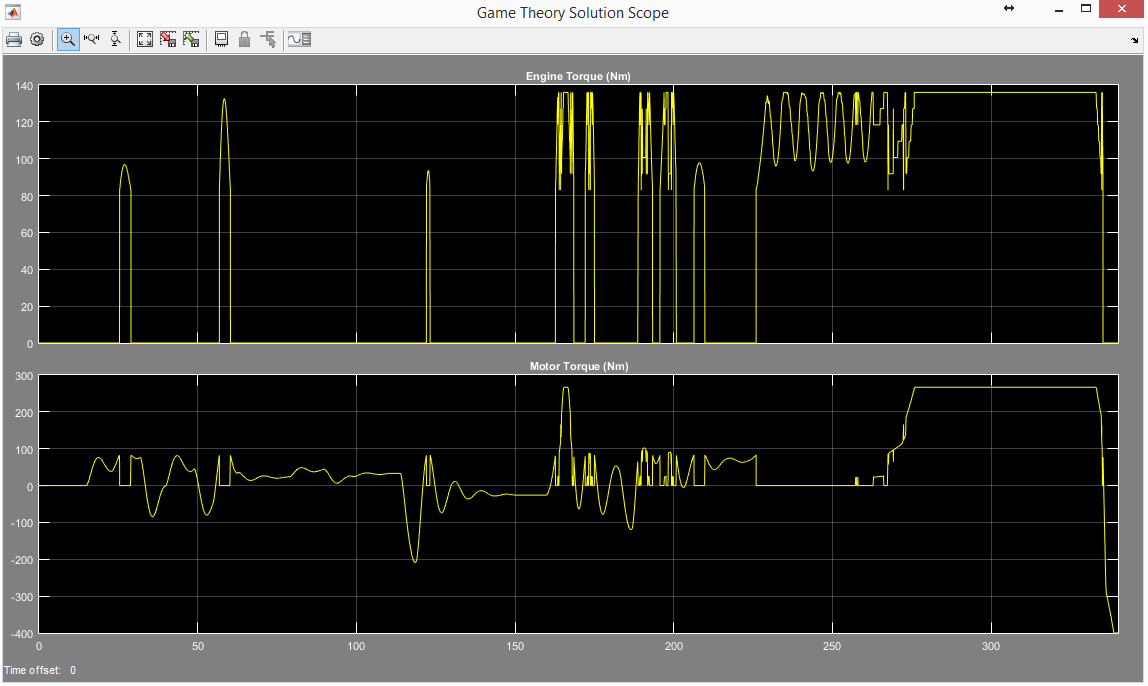
\includegraphics[scale=0.43]{figures/Pareto/FTP75-1/gameTheory30Juni}
\caption{Game Theory Scope with Pareto Optimality during FTP75-1}
\label{fig:gtpo1}

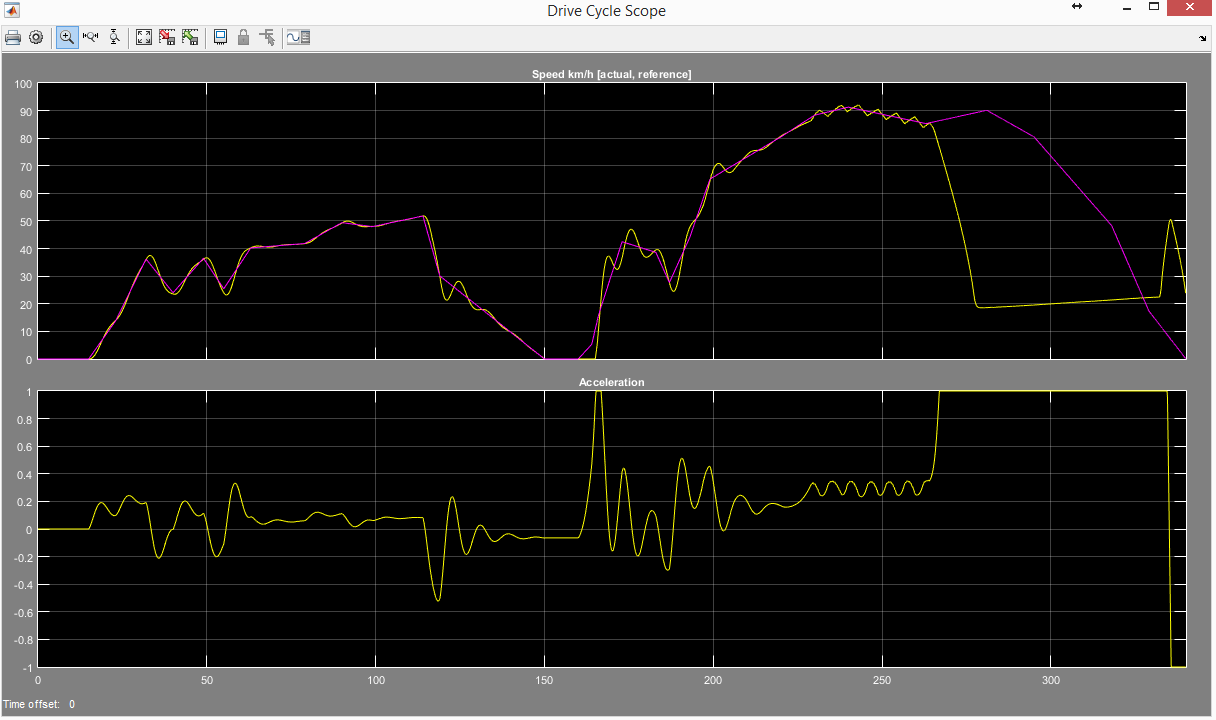
\includegraphics[scale=0.41]{figures/Pareto/FTP75-1/driveCycle30Juni}
\caption{Drive Cycle Scope with Pareto Optimality during FTP75-1}
\label{fig:dcpo1}
\end{figure}


\begin{figure}[hp]
\centering
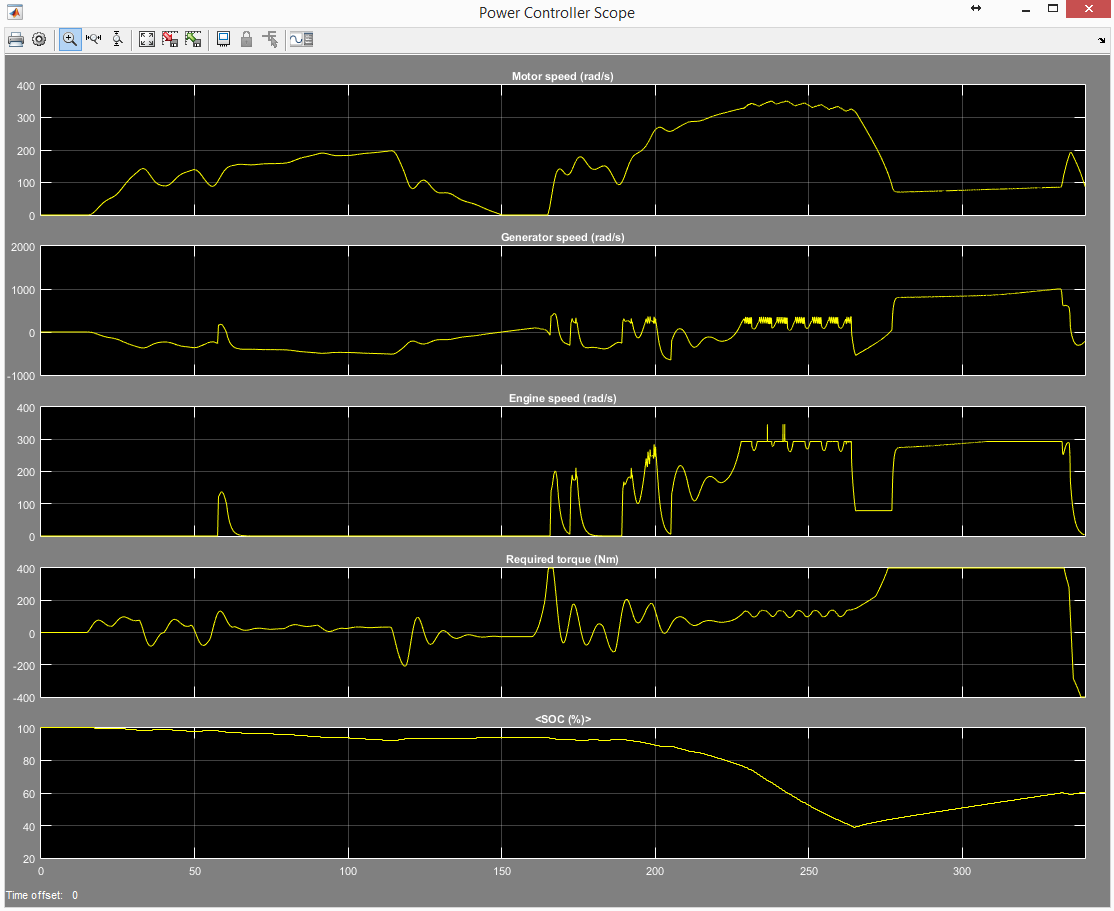
\includegraphics[scale=0.4]{figures/Pareto/FTP75-1/powerController30Juni}
\caption{Power Controller Scope with Pareto Optimality during FTP75-1}
\label{fig:pcpo1}

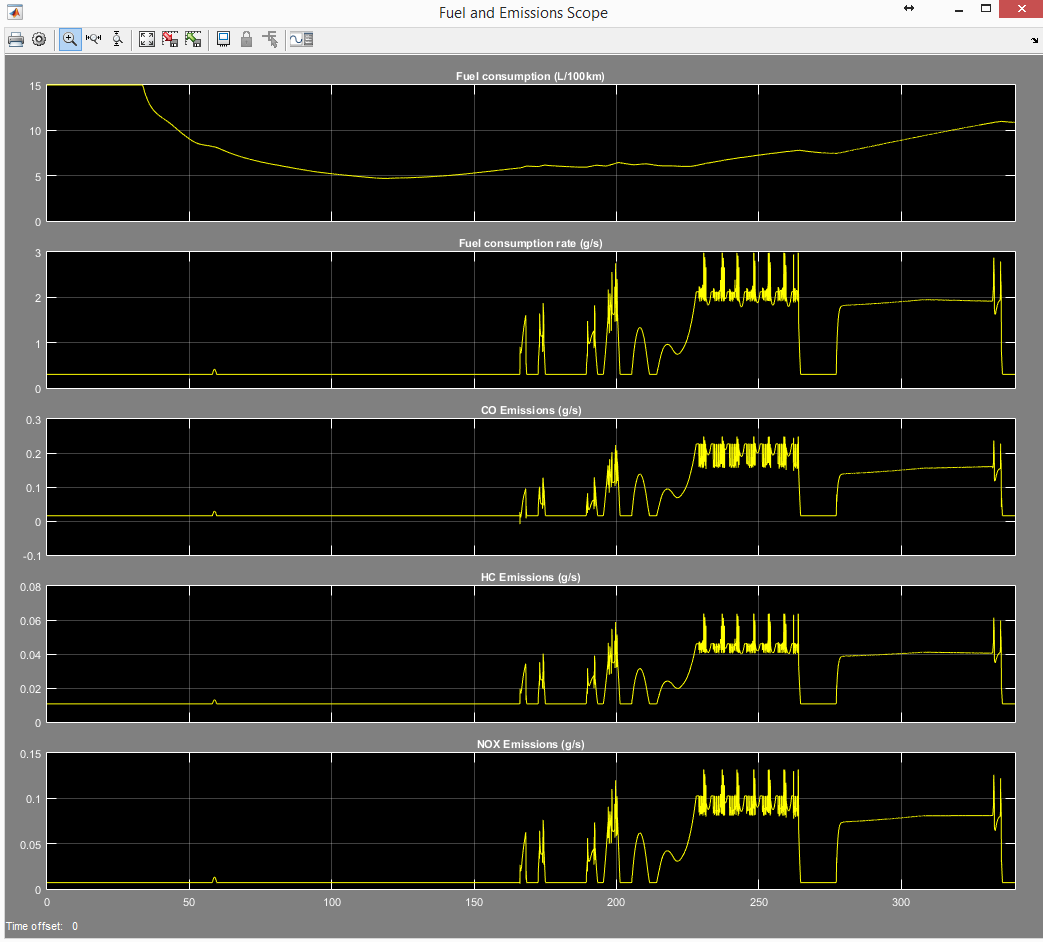
\includegraphics[scale=0.4]{figures/Pareto/FTP75-1/fuelEmissions30Juni}
\caption{Fuel and Emissions Scope with Pareto Optimality during FTP75-1}
\label{fig:fepo1}
\end{figure}


\begin{figure}[hp]
\centering
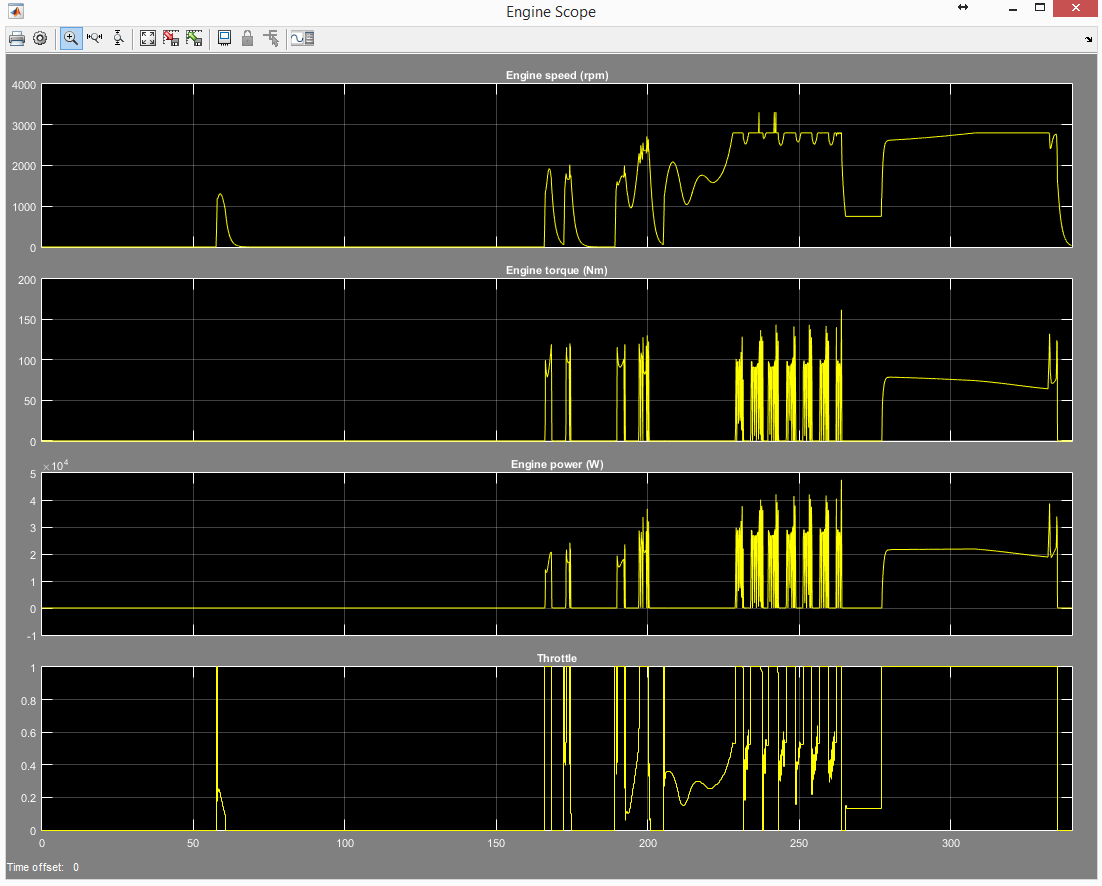
\includegraphics[scale=0.37]{figures/Pareto/FTP75-1/engine30Juni}
\caption{Engine Scope with Pareto Optimality during FTP75-1}
\label{fig:epo1}

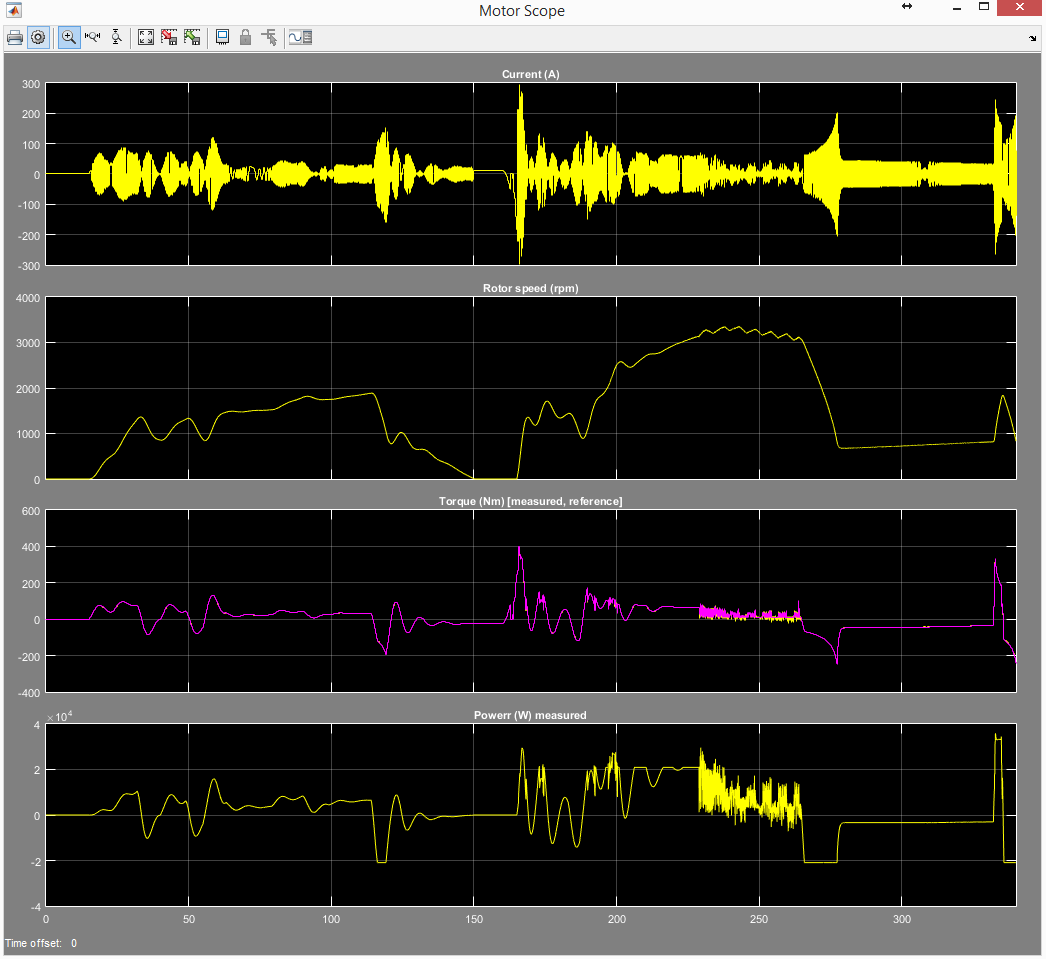
\includegraphics[scale=0.37]{figures/Pareto/FTP75-1/motor30Juni}
\caption{Motor Scope with Pareto Optimality during FTP75-1}
\label{fig:mpo1}
\end{figure}


The FTP75-2 results show that in the second phase of the drive cycle there is a much frequent switching on and off of the engine compared to the first phase. Moreover, the motor requests negative torque much more often. This is due to the fact that in Figure \ref{fig:dcpo2} there are more decelerations than in Figure \ref{fig:dcpo1} where the braking power is automatically used for recharging. Since the battery SOC does not fall below 40 \% and it does not have to be recharged purposefully in FTP75-2, the drive cycle demands are met very well and the actual and demanded speed are always close. Therefore, this phase also runs very fast compared to FTP75-1.

\begin{figure}[hp]
\centering
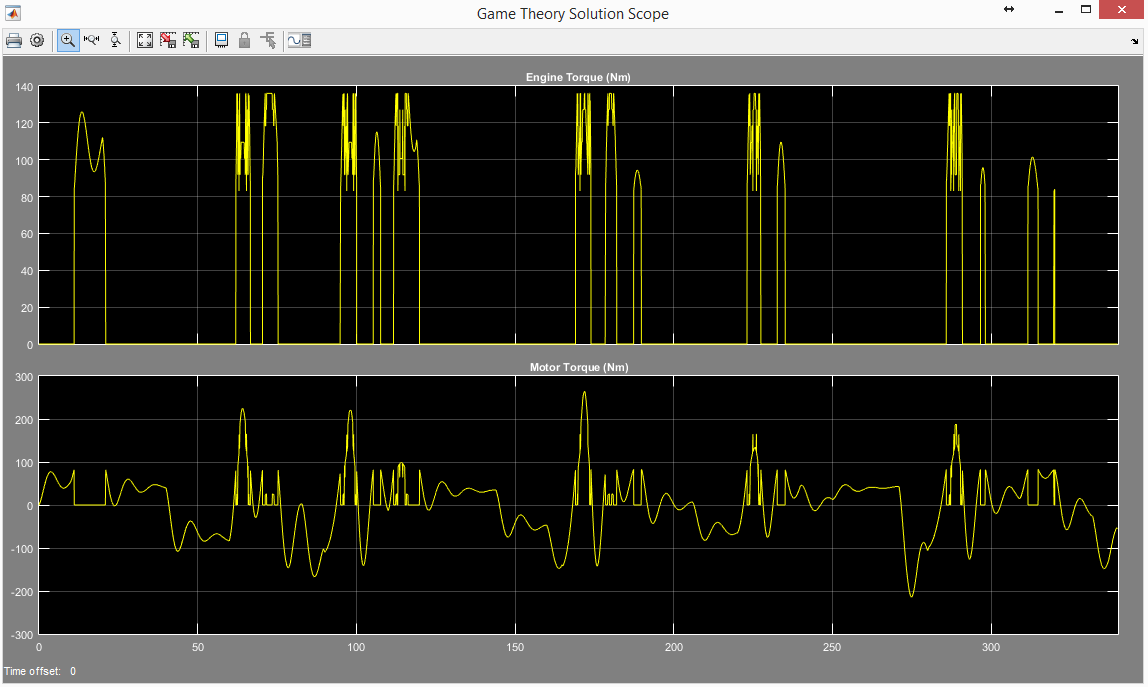
\includegraphics[scale=0.43]{figures/Pareto/FTP75-2/gameTheory03Juli}
\caption{Game Theory Scope with Pareto Optimality during FTP75-2}
\label{fig:gtpo1}

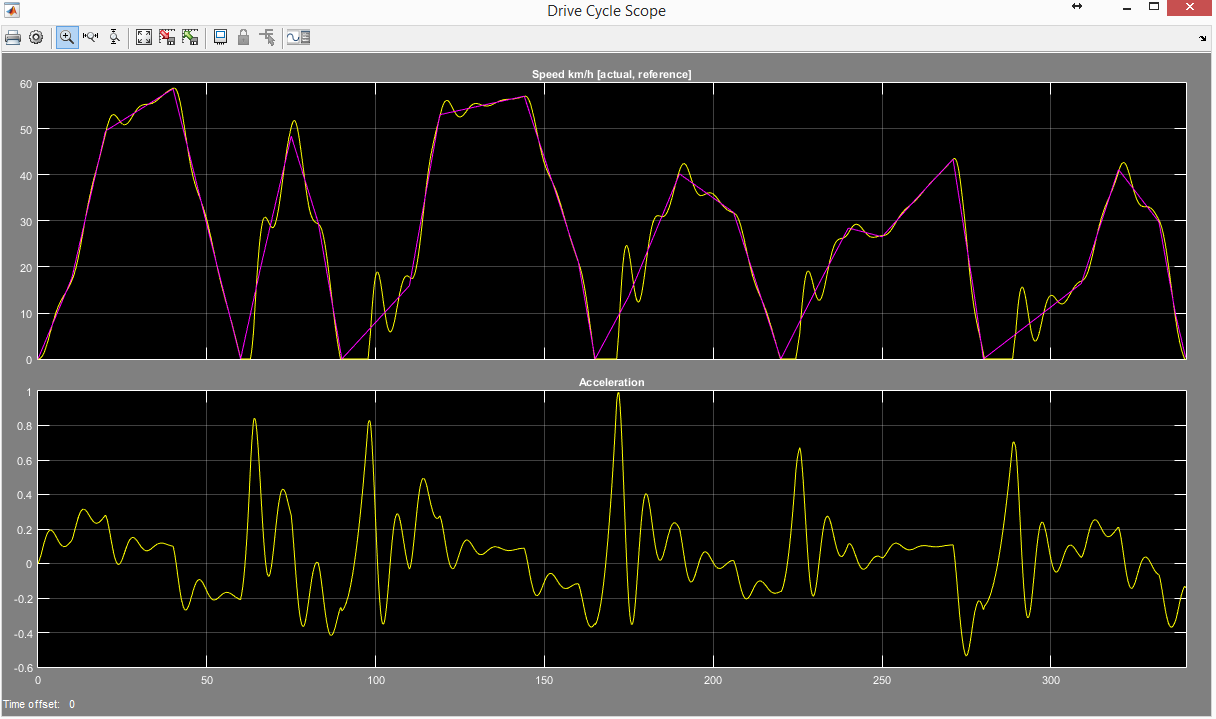
\includegraphics[scale=0.41]{figures/Pareto/FTP75-2/driveCycle03Juli}
\caption{Drive Cycle Scope with Pareto Optimality during FTP75-2}
\label{fig:dcpo1}
\end{figure}


\begin{figure}[hp]
\centering
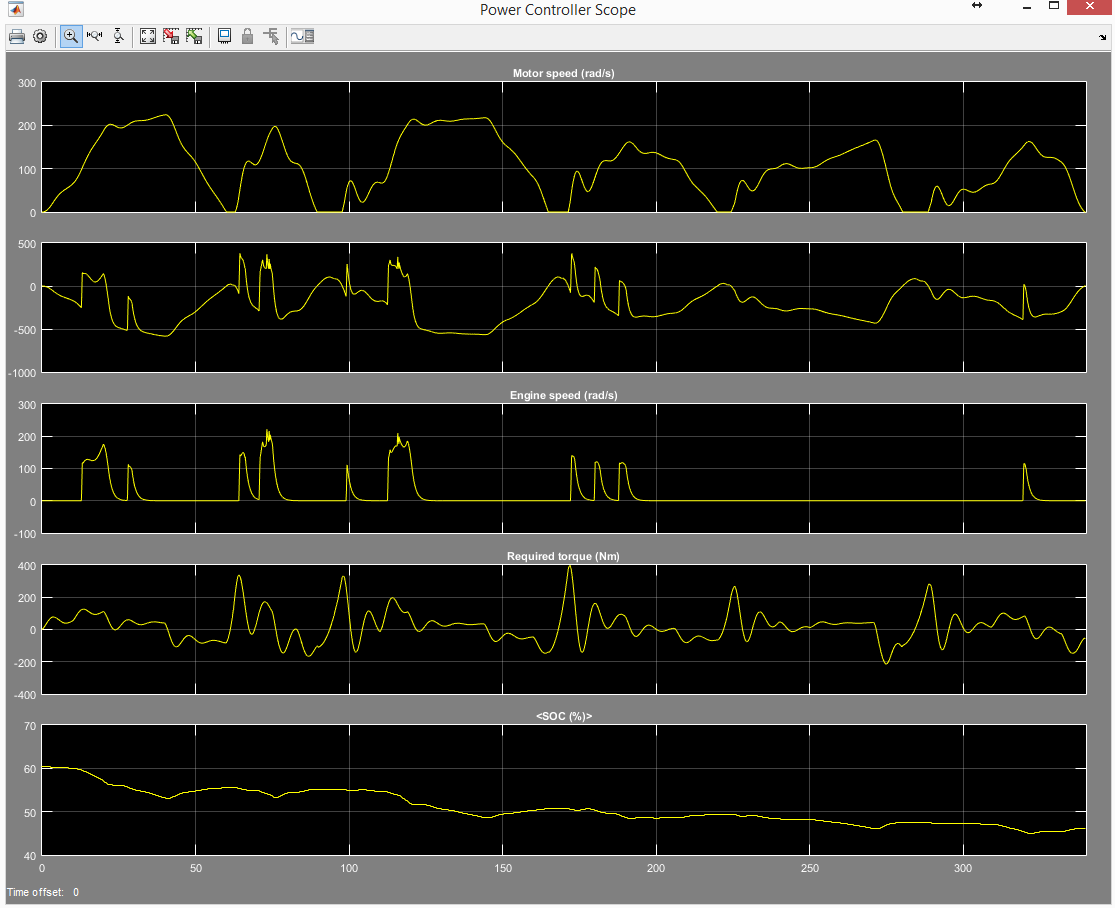
\includegraphics[scale=0.4]{figures/Pareto/FTP75-2/powerController03Juli}
\caption{Power Controller Scope with Pareto Optimality during FTP75-2}
\label{fig:pcpo1}

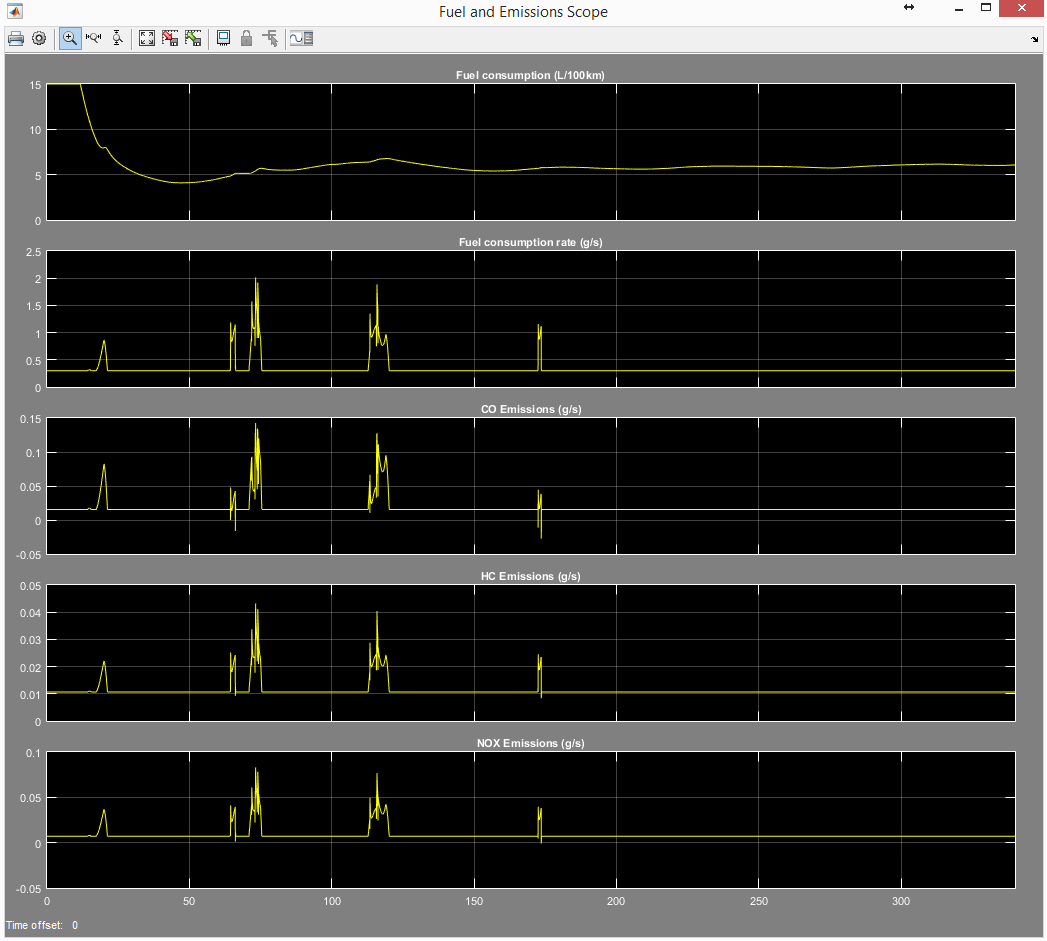
\includegraphics[scale=0.4]{figures/Pareto/FTP75-2/fuelEmissions03Juli}
\caption{Fuel and Emissions Scope with Pareto Optimality during FTP75-2}
\label{fig:fepo1}
\end{figure}


\begin{figure}[hp]
\centering
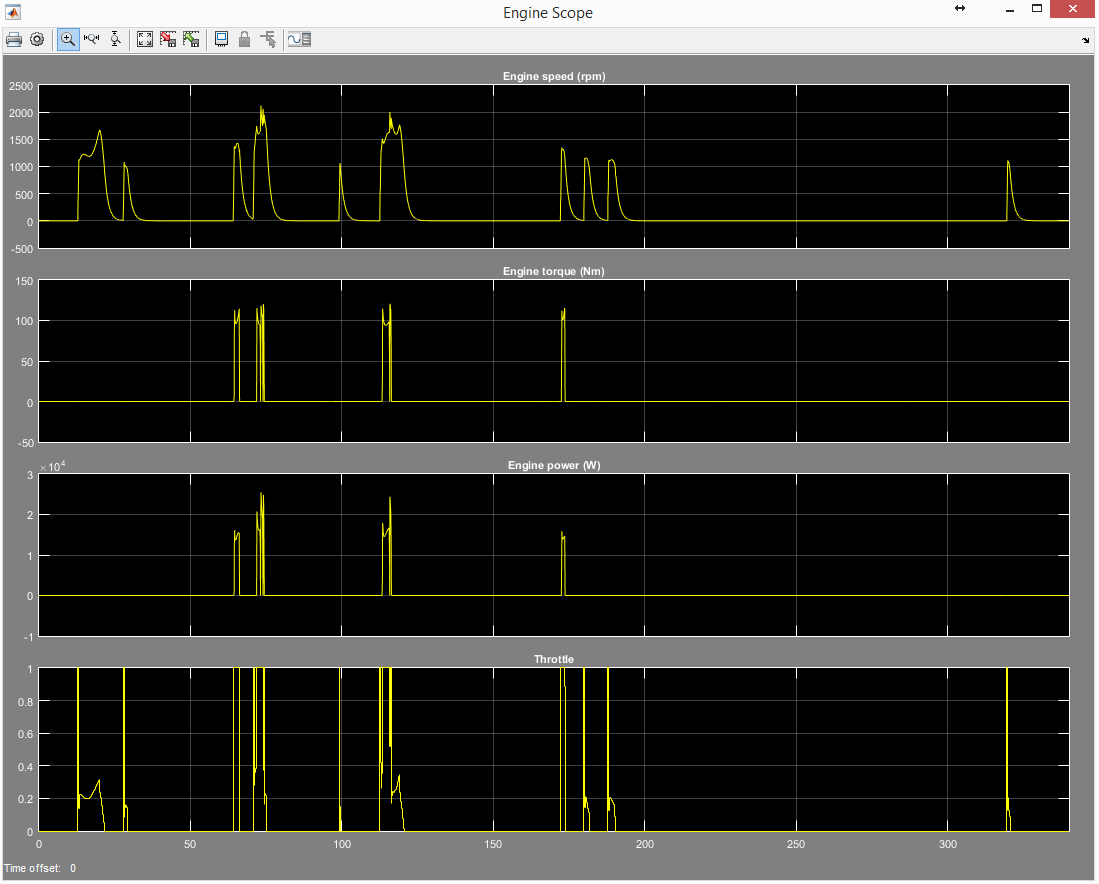
\includegraphics[scale=0.37]{figures/Pareto/FTP75-2/engine03Juli}
\caption{Engine Scope with Pareto Optimality during FTP75-2}
\label{fig:epo1}

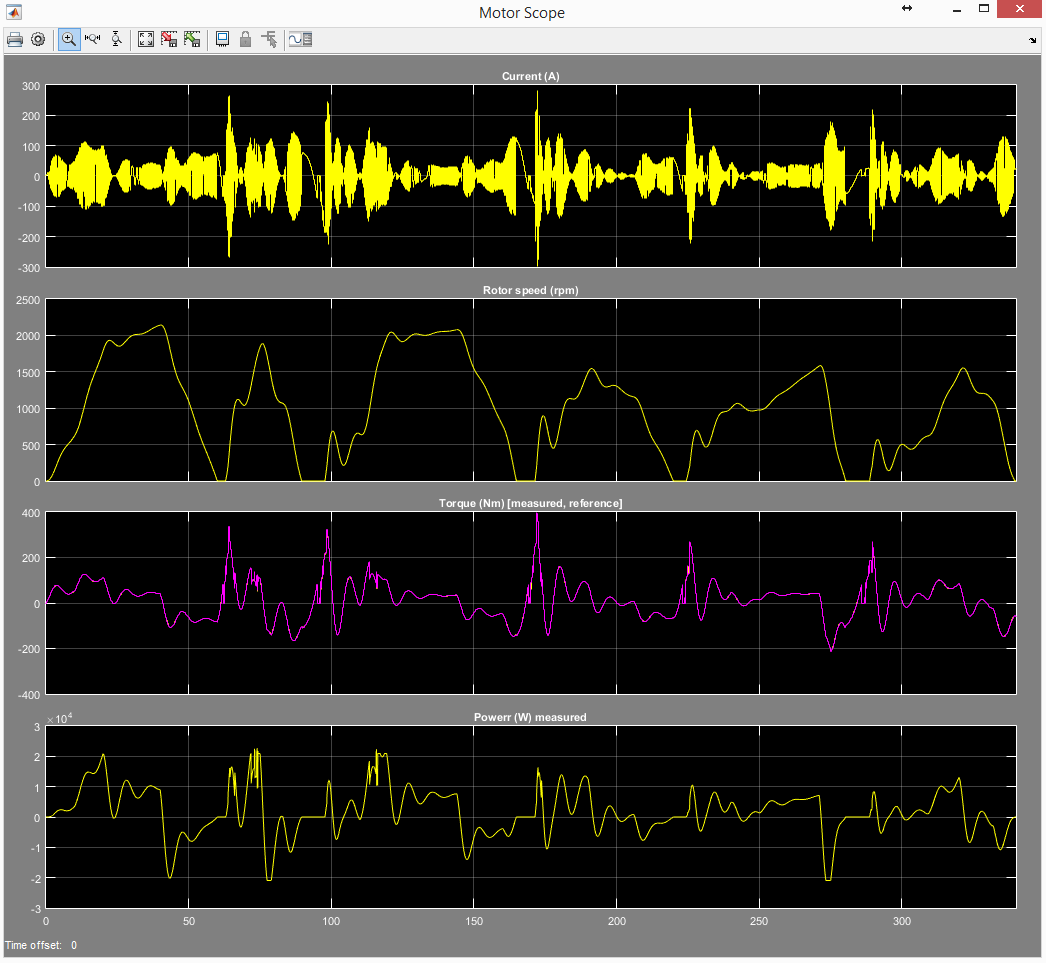
\includegraphics[scale=0.37]{figures/Pareto/FTP75-2/motor03Juli}
\caption{Motor Scope with Pareto Optimality during FTP75-2}
\label{fig:mpo1}
\end{figure}

In this phase the SOC again falls below 40 \% and then the difference between actual and demanded speed becomes at most 25 \textit{km/h}. This happens at time 120s and thus the acceleration is increased to the maximum of 1 and the required torque becomes 400 \textit{Nm}. During this time the engine and the motor are both prompted for torque constantly. When the battery is recharged to 60 \% at 180s, the actual speed still undergoes a lot of changes until it meets the required speed at time 240s. The reason is that the acceleration has been constantly 1 for a very long and then it suddenly drops to -1. The motor, engine and generator revolution speeds are also kept constant during recharge mode. Furthermore, in Figure \ref{fig:ene3} it can be seen that the problem with the rapid change of torque from the engine does not occur because there is no jittering of the engine revolution speed or torque.

In FTP75-4 similarly to the FTP75-2 the motor is prompted for negative torque much more frequently than the other phases FTP75-1 and FTP75-3 because there are more sudden accelerations and decelerations and the speed demand is changing more abruptly. It can be concluded that in this phase the drive cycle demands are again met very accurately like in FTP75-2, since there are almost no differences in the demanded and actual speeds in Figure \ref{fig:dcpo4}. The battery is both recharging during deceleration, corresponding to negative torque and discharging during acceleration with positive torque.

In the last phase, the FTP75-5, the battery has to be recharged in the 50s and the maximum difference of demanded and actual speed this incurs is 70 \textit{km/h}. During recharge mode the engine and motor are constantly contributing torque, because the torque demand is high. At 110s the maximum speed of this phase 85 \textit{km/h} is reached. At 120s the battery is already at the target 60 \% and the actual speed tries to keep up with the demanded speed. However, it goes up and down before it comes to the right demanded speed at 170s, similarly as in FTP75-3. After acceleration was kept constant, it takes time for it to adjust to the right amount and influence the actual speed correctly. After 170s the actual speed starts to meet eets the demand again. 

\subsection{Nash Equilibrium}
This section discusses the Game Theory Scope, Drive Cycle Scope, Power Controller Scope, Fuel Emissions Scope, Engine Scope and Motor Scope and the of all of the five phases in the FTP75 drive cycle when the game-theoretical solution is the Nash Equilibrium.

FTP75-1 results are displayed in the Figures \ref{fig:gtne1}, \ref{fig:dcne1}, \ref{fig:pcne1}, \ref{fig:fene1}, \ref{fig:ene1} and \ref{fig:mne1} in Appendix \ref{app:1}. The same problem with the jittering of the revolution speed and the torque of the engine is visible in \ref{fig:ene1}. At the end of the drive cycle phase the SOC is 60.5084 \%.

The FTP75-2 results are in Figure \ref{fig:gtne2}, \ref{fig:dcne2}, \ref{fig:pcne2}, \ref{fig:ene2} and \ref{fig:fene2}. 

The FTP75-3 results are shown in \ref{fig:gtne3}, \ref{fig:dcne3}, \ref{fig:pcne3}, \ref{fig:ene3} and \ref{fig:fene3}. 

The FTP75-4 results are in \ref{fig:gtne4}, \ref{fig:dcne4}, \ref{fig:pcne4}.

The FTP75-5 results are in \ref{fig:gtne5}, \ref{fig:dcne5}, \ref{fig:pcne5}.

For the next four game-theoretical approaches only the Game Theory scope will be shown, since there is little difference in the other scopes. Moreover, it is crucial to examine the motor and engine torque distribution differences between the different game theory approaches because that is the main topic in this thesis.

\subsection{Nash Bargaining solution}
The Nash Bargaining solution presented in Figure \ref{fig:gtns1} results are very similar to the Nash Equilibrium in Figure \ref{fig:gtne1}. Therefore, the FTP75 results of the Nash Bargaining solution will be primarily compared to the Nash Equilibrium results. The similarity is due to the fact that the Nash Equilibrium output was used for computing the Nash Equilibrium because it was taken as the conflict point as described in subsection \ref{subsec:nashbargFun}.

Despite the similarity, in FTP75-1 there is a difference at time from 160s to 170s in Figure \ref{fig:gtne1} where the Nash Equilibrium requests the maximum engine torque of 136 \textit{Nm} and then requests 115 \textit{Nm}, whereas in the Nash Bargaining solution in Figure \ref{fig:gtns1} after prompting for 136 \textit{Nm} it goes down to 90 \textit{Nm}. The same happens between 190s and 200s. Furthermore, the next difference is visible between 230s and 275s, where the motor torque is 0 and the engine torque in Nash Equilibrium is changing in the range from 128 to 100 \textit{Nm}. In the Nash Bargaining solution this also happens, but the change is more abrupt and it is either 128 or 100 \textit{Nm} rather than taking values in between them. Except for these cases, the game theory solutions with Nash Equilibrium and with Nash Bargaining solution are the same.

The FTP75-2 is also very similar to the Nash Equilibrium FTP75-2. At time 70-75s the Nash Bargaining solution requests again a wider range of torque from the engine, from 136 to 95 \textit{Nm}, while the Nash Equilibrium requests from 136 to only 110 \textit{Nm}. The same applies for the next peaks in Figure \ref{fig:gtns2}. Regarding the motor torque, the two solutions produce exactly the same output.

In the FTP75-3 drive cycle the results of the Nash Bargaining solution in \ref{fig:gtns3} are also similar to the Nash Equilibrium in Figure \ref{fig:gtne3}. The outline of the engine torque is the same with the difference that the Nash Bargaining solution requests a wide variety of torque in the upper range between 90 and 136 \textit{Nm}. The motor torque is again the same as in the Nash Equilibrium with exception that at time 185s there is a more sudden change than in the Nash Equilibrium solution, which corresponds  to the same time where the engine also undergoes a bigger change than in the Nash Equilibrium, which is seen from the thicker lines.

The same applies to the FTP75-4 drive cycle phase shown in Figure \ref{fig:gtns4}, where the Nash Bargaining solution gives a wider variety of engine torque output, while keeping the motor torque almost unchanged. However, at times 140s and 170s the motor torque of the Nash Bargaining solution is 125 \textit{Nm}, which is higher than in the Nash Equilibrium solution of 110 \textit{Nm}. This is due to the fact that the Nash Bargaining solution outputs engine torque in the range of 90 \textit{Nm} and 136, while the Nash Equilibrium only restricts it between 118 and 136 \textit{Nm}.

In the FTP75-5 the most obvious difference is that at time 120-125s the Nash Equilibrium produces torque between 110 and 136 \textit{Nm}, while the Nash Bargaining solution in Figure \ref{fig:gtns5} outputs a range of 95 to 136 \textit{Nm}. The same applies for the other peaks.

\subsection{Kalai-Smorodinsky solution}
The Kalai-Smorodinsky solution produces exactly the same results for the FTP75-1, FTP75-2 as the Nash solution does as shown in Figures \ref{fig:gtks1}, \ref{fig:gtks2}. The first visible difference between the two solutions appears in FTP75-3 at time 235-240s where the Kalai-Smorodinsky solution of the motor torque is going up and down from 0 to 90 repeatedly \textit{Nm}, while the Nash solution repeats this only 2 times - from 0 to 90, then to 0 and then to 90 again. This also affects the engine torque which behaves similarly in the range from 95 to 136 \textit{Nm} in the Kalai-Smorodinsky solution, but rather stays at 136 \textit{Nm} for the Nash solution. In the FTP75-4 there is no variation in comparison to the Nash Bargaining solution just as in the FTP75-5 where also no variation is visible. The almost identical results of the Kalai-Smorodinsky and the Nash solution come from fact that their concepts are very similar. Firstly, they both use the conflict point as a part of the computation. The Kalai-Smorodinksy solution is assumed to be an extension of the Nash solution, because it replaces one of the four axioms of the Nash solution with a new axiom for Individual Monotonicity and in addition takes into a account the ideal minimum payoff point.


\begin{table}[h]
\centering
\begin{tabular}{ |p{1.5cm}|p{1.5cm}|p{1.3cm}|p{1.3cm}|p{1.3cm}|p{1.3cm}|p{1.3cm}|p{1.3cm}|} 
 \hline
  \cline{3-8}
   & Drive cycle & \multicolumn{6}{|c|}{Game-theoretical solution} \\
   \cline{3-8}
   & & Pareto Optimality & Nash Equilibrium & Nash Solution & Kalai- Smorodinsky Solution & The Core & Shapley Value\\
 \hline\hline
 \multirow{5}{*}{\parbox{1.5cm}{Total fuel (l)}} 
 & FTP75-1 & & 0.406 & 0.397 & 0.397 & & \\ 
 & FTP75-2 & & 0.5635 & 0.554 & 0.554 & & \\  
 & FTP75-3 & & 0.901 & 0.893 & 0.893 & & \\ 
 & FTP75-4 & & 1.097 & 1.089 & 1.09 & & \\ 
 & FTP75-5 & & 1.566 & 1.543 & 1.513 & &\\ 
 \hline 
 \multirow{5}{*}{\parbox{1.5cm}{Fuel consumption (g/s)}} 
 & FTP75-1 & & 11.13 & 10.85 & 10.85 & &\\ 
 & FTP75-2 & & 6.109 & 6.082 & 6.082 & &\\ 
 & FTP75-3 & & 11.65 & 11.7 & 11.71 & & \\ 
 & FTP75-4 & & 6.384 & 6.384 & 6.384 & &\\ 
 & FTP75-5 & & 12.8 & 12.17 & 11.49 & & \\ 
 \hline 
 
 \multirow{5}{*}{\parbox{1.5cm}{CO (g/km)}} 
 & FTP75-1 & & 6.304 & 6.086 & 6.093 & & \\ 
 & FTP75-2 & & 2.334 & 2.328 & 2.328 & & \\ 
 & FTP75-3 & & 5.818 & 5.841 & 5.844 & & \\ 
 & FTP75-4 & & 2.361 & 2.361 & 2.361 & & \\ 
 & FTP75-5 & & 6.878 & 6.516 & 6.144 & & \\  
 \hline 
 
 \multirow{5}{*}{\parbox{1.5cm}{HC (g/km)}} 
 & FTP75-1 & & 1.979 & 1.937 & 1.938 & & \\ 
 & FTP75-2 & & 1.487 & 1.484 & 1.484 & & \\  
 & FTP75-3 & & 2.166 & 2.172 & 2.173 & & \\ 
 & FTP75-4 & & 1.636 & 1.636 & 1.636 & & \\ 
 & FTP75-5 & & 2.225 & 2.133 & 2.033 & & \\  
 \hline

 \multirow{5}{*}{\parbox{1.5cm}{NOX (g/km)}} 
 & FTP75-1 & & 3.113 & 3.011 & 3.014 & & \\
 & FTP75-2 & & 1.123 & 1.116 & 1.116 & & \\ 
 & FTP75-3 & & 2.975 & 2.989 & 2.992 & & \\ 
 & FTP75-4 & & 1.084 & 1.084 & 1.084 & & \\ 
 & FTP75-5 & & 3.511 & 3.321 & 3.119 & & \\ 
 \hline  
\end{tabular}
\caption{FTP75 fuel consumption and gas emissions}
\label{tab:fuelEmis}
\end{table}



\begin{table}[h]
\centering
\begin{tabular}{ |p{1.5cm}|p{1.5cm}|p{1.3cm}|p{1.3cm}|p{1.3cm}|p{1.3cm}|p{1.3cm}|p{1.3cm}|} 
 \hline
  \cline{3-8}
   & Drive cycle & \multicolumn{6}{|c|}{Game-theoretical solution} \\
   \cline{3-8}
   & & Pareto Optimality & Nash Equilibrium & Nash Solution & Kalai- Smorodinsky Solution & The Core & Shapley Value\\
 \hline\hline
 \multirow{5}{*}{\parbox{1.5cm}{Average speed (km/h)}}
 & FTP75-1 & & 38.63 & 38.79 & 38.77 & & \\
 & FTP75-2 & & 27.27 & 27.27 & 27.27 & & \\ 
 & FTP75-3 & & 29.84 & 29.83 & 29.83 & & \\ 
 & FTP75-4 & & 23.48 & 23.48 & 23.48 & & \\ 
 & FTP75-5 & & 29.84 & 29.83 & 29.83 & & \\ 
 \hline 
 \multirow{5}{*}{\parbox{1.5cm}{Total distance (km)}}
 & FTP75-1 & & 3.648 & 3.664 & 3.661 & & \\ 
 & FTP75-2 & & 2.576 & 2.576 & 2.676 & & \\ 
 & FTP75-3 & & 2.901 & 2.901 & 2.9 & & \\ 
 & FTP75-4 & & 3.066 & 3.066 & 3.066 & & \\ 
 & FTP75-5 & & 3.664 & 3.73 & 3.083 & & \\ 
 \hline 
 \multirow{5}{*}{\parbox{1.5cm}{Final SOC (\%)}}
 & FTP75-1 & & 60.508 & 60.554 & 60.54 & & \\ 
 & FTP75-2 & & 46.494 & 46.422 & 46.408 & & \\ 
 & FTP75-3 & & 56.953 & 56.933 & 56.9809 & & \\ 
 & FTP75-4 & & 41.929 & 41.927 & 41.975 & & \\ 
 & FTP75-5 & & 49.141 & 46.955 & 42.871 & & \\ 
 \hline

 \hline
\end{tabular}
\caption{FTP75 speed, distance and battery}
\label{tab:fuelEmis}
\end{table}
